\section{Introduce}

%------------------------------------------------
\begin{frame}[fragile]{RS-485原理}

  \begin{itemize}
    \item RS485通过2根信号线传输数据。
    \item 逻辑“1”以两线间的电压差为+(2—6)V表示;逻辑
    “0”以两线间的电压差为-(2—6)V表示。
    \item  可以在汇流排上进行联网实现多机通信,汇流排上允许挂
    多个收发器,从现有的RS485晶片来看,有可以挂32、
    64、128、256等不同个设备的驱动器。
  \end{itemize}

\begin{figure}[htbp]
\begin{center}
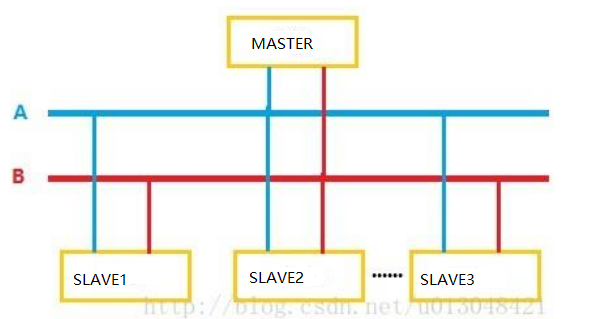
\includegraphics[width=6cm]{img/485net}
\caption{BAN }
\label{Overview}
\end{center}
\vspace{-0.5em}
\end{figure}


\end{frame}


%------------------------------------------------
\begin{frame}[fragile]{RS-485特点}

\begin{itemize}
  \item RS485通信速度快,资料最高传输速率为10Mbps以上
  \item RS485内部的物理结构,采用的是平衡驱动器和查分接收
  器的组合,抗干扰能力大大增加。
  \item  传输速率最远可达到1200米左右,使用中继可以传输更
  远距离。
\end{itemize}

\end{frame}

%------------------------------------------------
\begin{frame}[fragile]{产生时钟偏差的原因}

\begin{itemize}
  \item 初始绝对时钟不同:不同系统启动之後的初始绝对时间有
  差异
  \item 不同系统的时钟脉冲有细微差异,该差异导致绝对时钟产
  生累积误差
\end{itemize}

\end{frame}

%------------------------------------------------
\begin{frame}[fragile]{RS-485时钟同步原理-HW基础}

\begin{itemize}
  \item 如果需要MCU间的时钟同步,需要在Master和Slave之间
增加一条时钟线,Master在该时钟线上产生同步时钟方波。
\end{itemize}

\begin{figure}[htbp]
\begin{center}
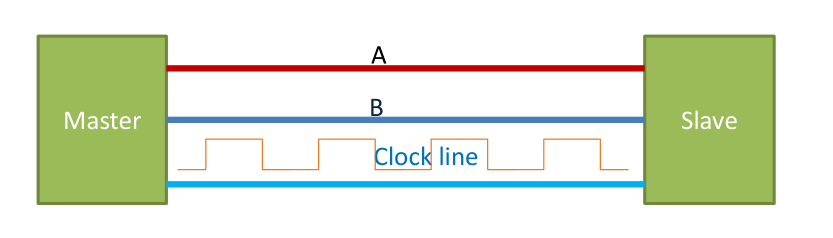
\includegraphics[width=6cm]{img/syncchart}
\caption{BAN }
\label{Overview}
\end{center}
\vspace{-0.5em}
\end{figure}
\end{frame}




%------------------------------------------------
\begin{frame}[fragile]{RS-485时钟同步原理-初始时间同步}

\begin{itemize}
  \item Master启动本地时钟,在时钟线上产生方波信号。
\item 在第一个方波信号的上升沿获取本地RTC绝对时间T 0 , 并
通过RS-485把该时间发送到Slave端
\item Slave收到方波上升沿开始计数
\item Slave收到Master发送过来的绝对时间之后,把本地RTC时间设置为T0
\end{itemize}

\begin{figure}[htbp]
\begin{center}
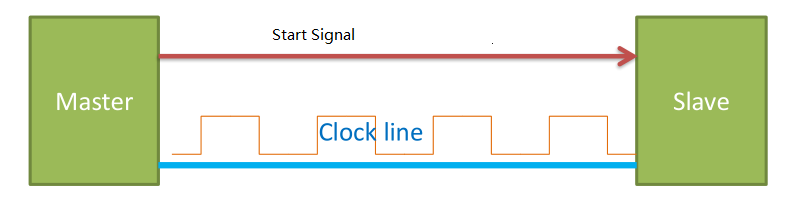
\includegraphics[width=6cm]{img/abstim}
\caption{BAN }
\label{Overview}
\end{center}
\vspace{-0.5em}
\end{figure}
\end{frame}





%------------------------------------------------
\begin{frame}[fragile]{RS-485时钟同步原理-延迟校准}
  Slave设置本地RTC绝对时间为T后,由於RS-485传输延迟和
  本地SW解析数据时间,Slave绝对时间和Master相比会有一
  定延迟,该延迟通过时钟线产生的方波进行校准,具体方法
  如下:
\begin{itemize}
  \item Slave端设置完成本地RTC绝对时间T 0 之後,等待下一次时
  钟上升沿。
\item 收到时钟上升沿之後,假设收到的是第N 0 个时钟上升沿.
重新设置本地绝对时间为:T 0 +N 0 *t. 设置完成後,Slave
绝对时间和Master绝对时间完成同步。

\end{itemize}

Note:t是时钟方波一个周期时长。


\end{frame}




%------------------------------------------------
\begin{frame}[fragile]{RS-485时钟同步原理-延迟校准}

  \begin{figure}[htbp]
  \begin{center}
  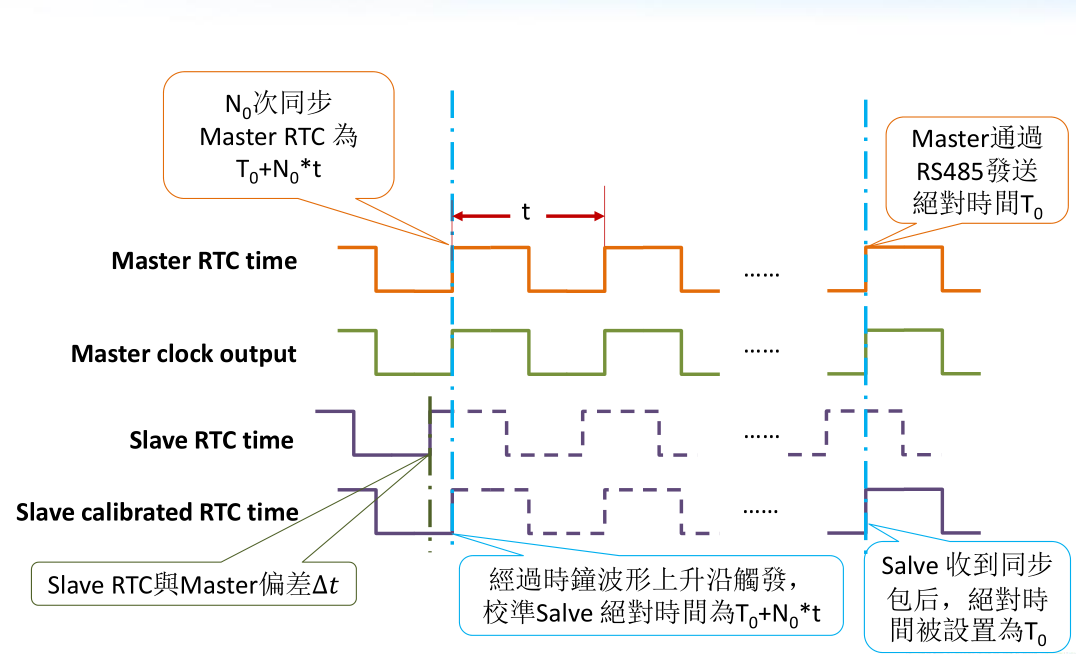
\includegraphics[width=10cm]{img/delay1}
  \caption{BAN }
  \label{Overview}
  \end{center}
  \vspace{-0.5em}
  \end{figure}

\end{frame}




%------------------------------------------------
\begin{frame}[fragile]{RS-485时钟同步原理- 时钟累积误差校准}
  Slave和Master时间完成同步后,由於两个系统有独立的时
钟脉冲,双方时钟脉冲会有误差从而导致绝对时间产生累误
差,该误差同样通过时钟方波进行校准,方法如下:


\begin{itemize}
  \item  每次Slave设置完成RTC绝对时间后,都记录该时间T并对
  方波重新计数.
\item Slave每隔N个方波都重新设置本地RTC时间为T+N*t,从
而消除累积误差。


\end{itemize}

Note:t是时钟方波一个周期时长。

\end{frame}

%------------------------------------------------
\begin{frame}[fragile]{Our Design}
我们BAN 的原本设计是这样的:
\begin{figure}[htbp]
\begin{center}
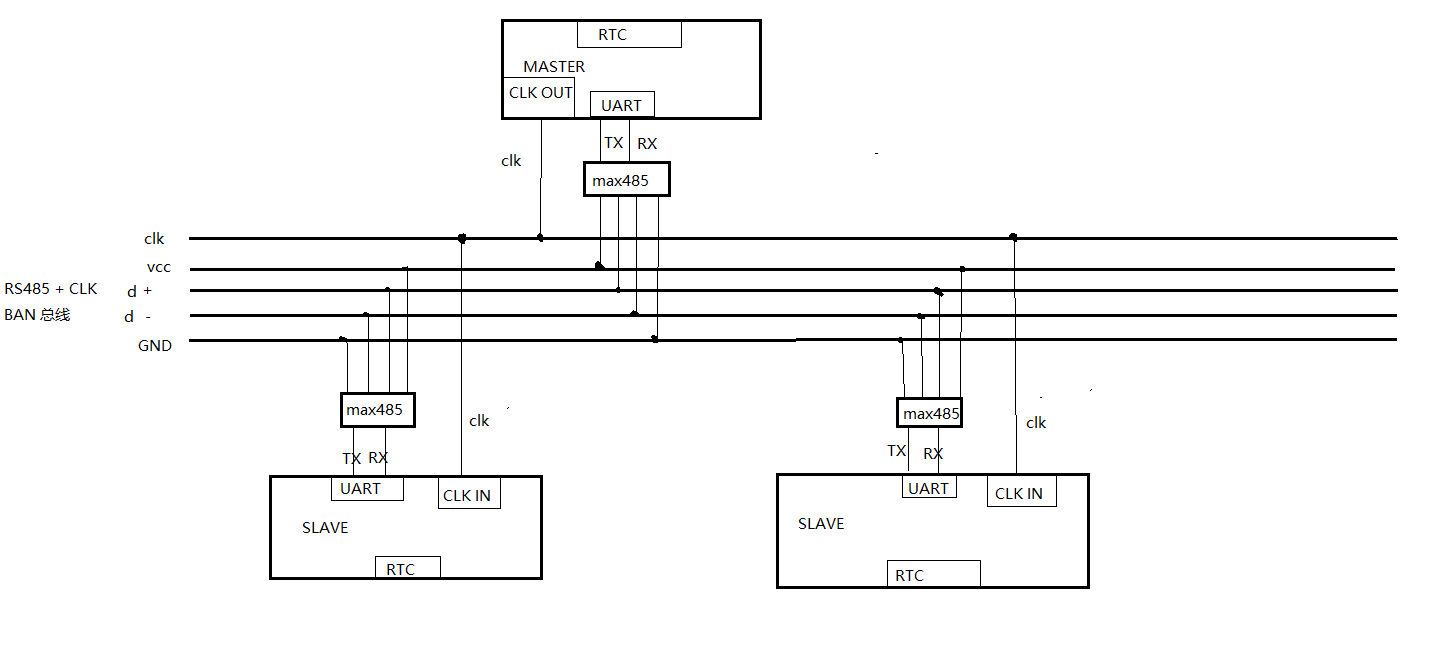
\includegraphics[width=10cm]{img/overview}
\caption{BAN }
\label{Overview}
\end{center}
\vspace{-0.5em}
\end{figure}
\end{frame}





%------------------------------------------------
\begin{frame}[fragile]{BUS}
1. 由 RS485 增添一根 clk线 形成 BAN 总线的 基本硬件线路。

2. clk 用于产生 ms 级别的脉冲波,用于时钟的同步。

3.  d+ d- 是差分处理后的数据信号。

图\ref{Overview} 假设了 挂载在总线上的设备有一个主机,两个从机。

\end{frame}

%------------------------------------------------
\begin{frame}[fragile]{UART \& 485}

max485 是一型 RS232 转 RS485 的芯片,可以把串口数据 转化为 差分信号,使其符合\textbf{RS-485}
电气规范。

STM32 方面需要实现串口的驱动,使确保串口可以实时的发送数据。接收数据。

\end{frame}

%------------------------------------------------
\begin{frame}[fragile]{RTC \& CLK}
本地时钟用于本地计数,同步时钟用于同步BAN 上设备的时钟。
\begin{itemize}
\item  RTC ,本地时钟。 每个设备都有个本地时钟。 计时粒度为 100us.

\item  CLK,同步时钟。 BAN总线上的设备使用时钟线来完成时钟同步。主设备的定时器产生同步脉冲,从设备
的定时器捕获同步脉冲完成同步。
\end{itemize}


\end{frame}


%------------------------------------------------
\begin{frame}[fragile]{Demo}

在demo 中,为了克服硬件条件的限制,我们:
\begin{itemize}
    \item 没有使用max485 来完成\textbf{TTL信号}转\textbf{差分信号}.
    \item 使用另外的一个定时器来模拟RTC的功能。
    \item 只能模拟一个主设备,一个从设备的情况。
    \item 使用串口发送开始信号
\end{itemize}

\end{frame}


%------------------------------------------------
\begin{frame}[fragile]{Demo 连线}

下图是demo 的连线和结构图:
\begin{figure}[htbp]
\begin{center}
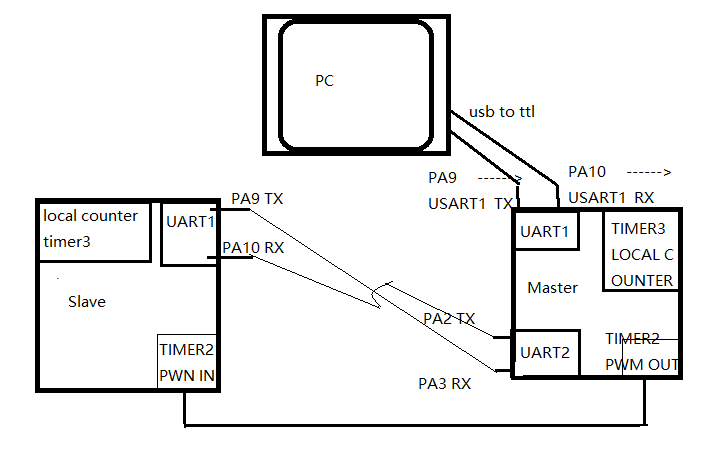
\includegraphics[width=10cm]{img/demo0}
\caption{demo}
\label{Overview}
\end{center}
\vspace{-0.5em}
\end{figure}

\end{frame}
